% originally gnbvig.Rnw, from James Probets' project
\documentclass[article,nojss]{jss}
\usepackage{amsmath, amsfonts}

%% need no \usepackage{Sweave}
%\VignetteIndexEntry{Garch and white noise tests}


\author{James Proberts\\University of Manchester \And
        Georgi N. Boshnakov \\ University of Manchester
}
\Plainauthor{James Proberts and Georgi N. Boshnakov}


\title{ARMA-GARCH modelling and white noise tests}
\Plaintitle{Garch modelling and white noise tests}
%\Shorttitle{} %% a short title (if necessary)

%% an abstract and keywords
\Abstract{
  This vignette illustrates applications of white noise tests in GARCH
  modelling. It is based on an example from an MMath project by the first author.
}
\Keywords{autocorrelations, white noise tests, IID tests, GARCH models, time series}

\Plainkeywords{autocorrelations, white noise tests, IID tests, GARCH models, time series}


%% publication information
%% NOTE: Typically, this can be left commented and will be filled out by the technical editor
%% \Volume{50}
%% \Issue{9}
%% \Month{June}
%% \Year{2012}
%% \Submitdate{2012-06-04}
%% \Acceptdate{2012-06-04}
%% The address of (at least) one author should be given
%% in the following format:
\Address{
  Georgi N. Boshnakov\\
  School of Mathematics\\
  The University of Manchester\\
  Oxford Road, Manchester M13 9PL, UK\\
  URL: \url{http://www.maths.manchester.ac.uk/~gb/}
}


\begin{document}
%% include your article here, just as usual
%% Note that you should use the \pkg{}, \proglang{} and \code{} commands.

% borrowed from zoo.Rnw in package zoo:


%\VignetteIndexEntry{Brief guide to package sarima}
%\VignetteDepends{}
%\VignetteKeywords{portmanteau tests, autocorrelations, ARIMA, time series, S4, R}
%\VignettePackage{sarima}






%\VignetteIndexEntry{Brief guide to package sarima}
%\VignetteDepends{}
%\VignetteKeywords{portmanteau tests, autocorrelations, ARIMA, time series, S4, R}
%\VignettePackage{sarima}


\section{The data}

In this example we consider data from Freddie Mac, a mortgage loan company in
the USA. This stock is an interesting case for study. In the financial crash of
2008 it dropped from roughly \$60 to \$0.5 over the course of a year. It is now
(April 2017) majority owned by the government and has all its profits and
dividends sweeped. There has been speculation on this stock being returned to
private ownership for years making it prone to clusters of volatility.

We import weekly data from Yahoo Finance covering the period from
10/05/2006 to 22/04/2017, and calculate the weekly simple log returns.
%% 2019-09-12: removing rev() from logreturns <-
%%    diff(rev(log(FMCC$FMCC.Close))) I hadn't noticed that James had
%%    done this!  Though the GARCH models are not reversible in the
%%    way the ARMA models are, the results and their interpretation
%%    don't change materially in this case since here only the sign of
%%    the returns is flipped
\begin{Schunk}
\begin{Sinput}
R> ## using a saved object, orginally imported with:
R> ##  FMCC <- yahooSeries("FMCC", from = "2006-05-10", to = "2017-04-22",
R> ##                         freq = "weekly")
R> FMCC <- readRDS(system.file("extdata", "FMCC.rds", package = "sarima"))
R> logreturns <- diff(log(FMCC$FMCC.Close))
\end{Sinput}
\end{Schunk}
A plot of the log-returns. is given in Fig.~1.
\begin{figure}[ht]
  \centering
\begin{Schunk}
\begin{Sinput}
R> plot(logreturns, type="l", main="Log-returns of FMCC")
\end{Sinput}
\end{Schunk}
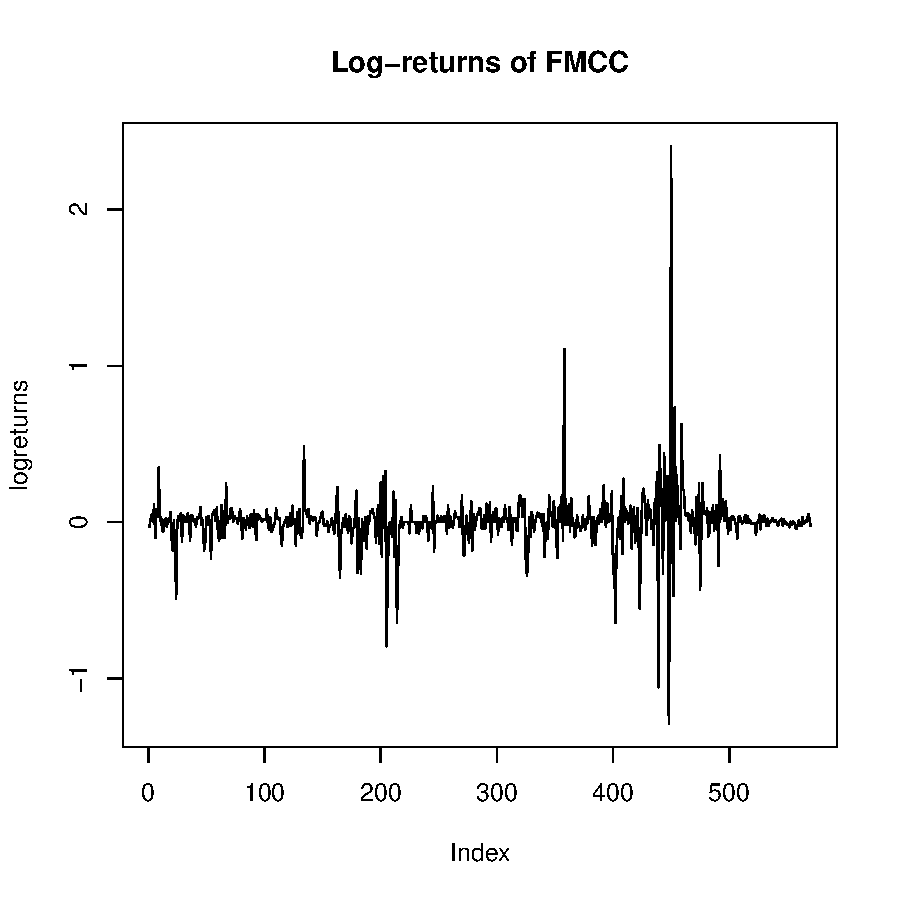
\includegraphics{garch_tests_example-004}
\caption{Log-returns of weekly log-returns of FMCC from 10 May 2006 to 22 Apr 2017.}
\end{figure}
We also calculate the autocorrelations and partial autocorrelations for the log returns.
\begin{Schunk}
\begin{Sinput}
R> FMCClr.acf <- autocorrelations(logreturns)
R> FMCClr.pacf <- partialAutocorrelations(logreturns)
\end{Sinput}
\end{Schunk}

\section{Autocorrelations}
\label{sec:autocorrelations}

We now produce a plot of the autocorrelations to assess whether the series is autocorrelated,
see Fig.~2. There are two bounds plotted on the graph. The straight red line represents the
standard bounds under the strong white noise assumption. The second line is under the
hypothesis that the process is GARCH.
% plot(FMCClr.acf, data = logreturns,
%      main="Autocorrelation test of the log returns of FMCC")
\begin{figure}[ht]
  \centering
\begin{Schunk}
\begin{Sinput}
R> plot(FMCClr.acf, data = logreturns)
\end{Sinput}
\end{Schunk}
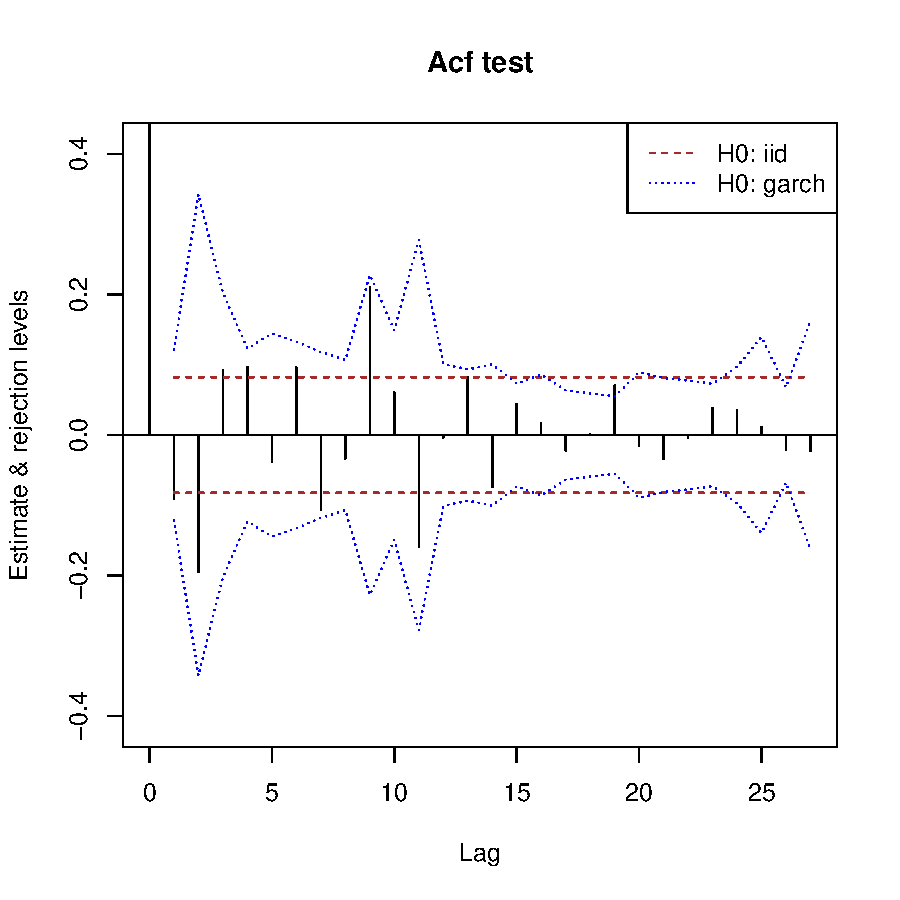
\includegraphics{garch_tests_example-006}
\caption{Autocorrelation test of the log returns of FMCC}
\end{figure}

Several autocorrelations seem significant under the iid hypothesis.
This may lead us to fitting an ARMA or ARMA-GARCH model.
On the other hand, the autocorrelations are well into the bands produced under the GARCH
hypothesis, suggesting a pure GARCH model,
without any ARMA terms.
So, it matters on which test we base our decision.

The partial autocorrelation function can be used instead of the autocorrelations, with
similar inferences, see Fig.~3.
\begin{figure}
  \centering
\begin{Schunk}
\begin{Sinput}
R> plot(FMCClr.pacf, data = logreturns,
+ main="Partial Autocorrelation test of the log returns of FMCC")
\end{Sinput}
\end{Schunk}
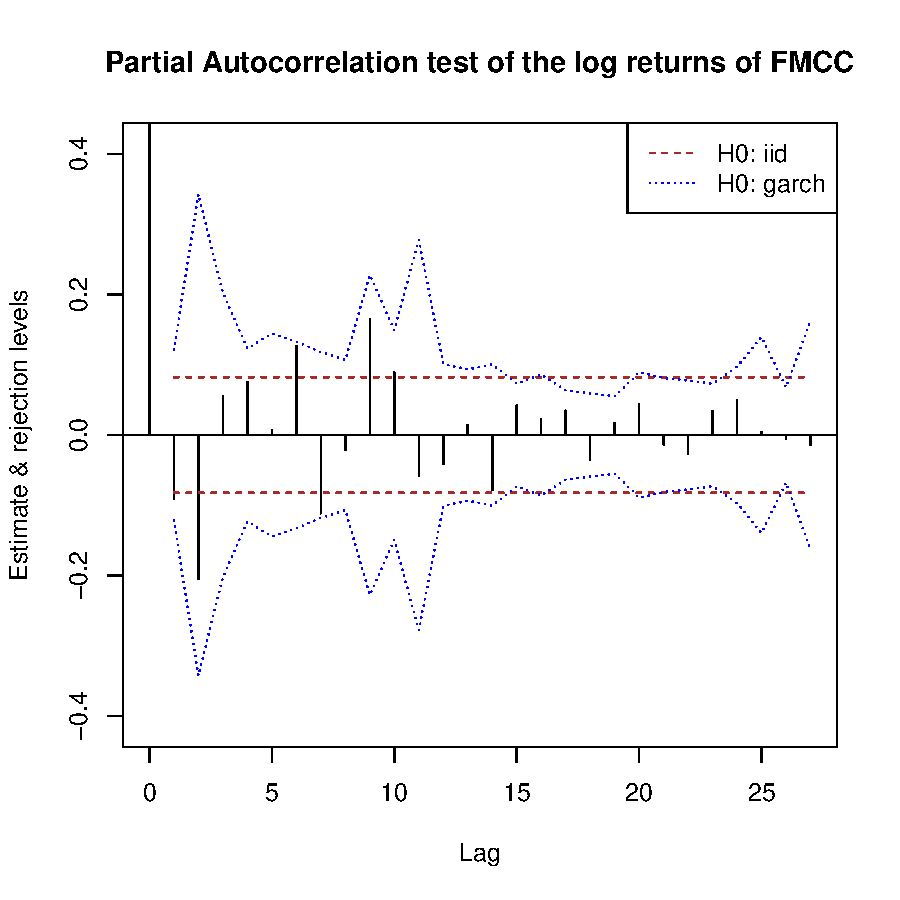
\includegraphics{garch_tests_example-007}
\end{figure}


\section{Pormanteau tests}
\label{sec:white-noise-tests}


Routine portmanteau tests, such as Ljung-Box, also reject the IID hypothesis.
Here we carry out IID tests using the method of Li-McLeod:
\begin{Schunk}
\begin{Sinput}
R> wntLM <- whiteNoiseTest(FMCClr.acf, h0 = "iid", nlags = c(5,10,20),
+                         x = logreturns, method = "LiMcLeod")
R> wntLM$test
\end{Sinput}
\begin{Soutput}
         ChiSq DF       pvalue
[1,]  37.18469  5 5.499929e-07
[2,]  76.99131 10 1.946524e-12
[3,] 103.19392 20 3.363466e-13
attr(,"method")
[1] "LiMcLeod"
\end{Soutput}
\end{Schunk}
Small p-values lead to rejection of the null hypothesis at reasonable levels.
Rejection of the null hypothesis is often taken to mean that the data are autocorrelated.

Let us test for fitting a GARCH-type model by using the following code which has the
weaker assumption that the log returns are GARCH.
Let us change the null hypothesis to "garch" (one possible weak white noise hypothesis):
\begin{Schunk}
\begin{Sinput}
R> wntg <- whiteNoiseTest(FMCClr.acf, h0 = "garch", nlags = c(5,10,15), x = logreturns)
R> wntg$test
\end{Sinput}
\begin{Soutput}
      h         Q      pval
[1,]  5  4.338367 0.5017961
[2,] 10 10.318035 0.4130480
[3,] 15 16.522535 0.3481985
\end{Soutput}
\end{Schunk}

The high p-values give no reason to reject the hypothesis
that the log-returns are a GARCH white noise process. In other words, there is no need to
ARMA modelling.



\section{Fitting GARCH(1,1) models and their variants}
\label{sec:fit garch}

Based on the discussion above, we go on to fit GARCH model(s), starting with a GARCH(1,1)
model with Gaussian innovations.

\begin{Schunk}
\begin{Sinput}
R> fit1 <- garchFit(~garch(1,1), data = logreturns, trace = FALSE)
R> summary(fit1)
\end{Sinput}
\begin{Soutput}
Title:
 GARCH Modelling 

Call:
 garchFit(formula = ~garch(1, 1), data = logreturns, trace = FALSE) 

Mean and Variance Equation:
 data ~ garch(1, 1)
<environment: 0x55d0f69aebf0>
 [data = logreturns]

Conditional Distribution:
 norm 

Coefficient(s):
      mu     omega    alpha1     beta1  
0.006865  0.001658  1.000000  0.328690  

Std. Errors:
 based on Hessian 

Error Analysis:
        Estimate  Std. Error  t value Pr(>|t|)    
mu     0.0068650   0.0031504    2.179  0.02933 *  
omega  0.0016580   0.0005068    3.271  0.00107 ** 
alpha1 1.0000000   0.1452152    6.886 5.72e-12 ***
beta1  0.3286902   0.0797419    4.122 3.76e-05 ***
---
Signif. codes:  0 ‘***’ 0.001 ‘**’ 0.01 ‘*’ 0.05 ‘.’ 0.1 ‘ ’ 1

Log Likelihood:
 450.174    normalized:  0.789779 

Description:
 Tue Mar 14 16:07:59 2023 by user: georgi 


Standardised Residuals Tests:
                                Statistic p-Value   
 Jarque-Bera Test   R    Chi^2  900.8757  0         
 Shapiro-Wilk Test  R    W      0.9106544 0         
 Ljung-Box Test     R    Q(10)  13.256    0.2097087 
 Ljung-Box Test     R    Q(15)  22.14342  0.104098  
 Ljung-Box Test     R    Q(20)  33.05104  0.03330812
 Ljung-Box Test     R^2  Q(10)  5.628762  0.8454295 
 Ljung-Box Test     R^2  Q(15)  5.999129  0.9797624 
 Ljung-Box Test     R^2  Q(20)  10.00362  0.9681062 
 LM Arch Test       R    TR^2   5.275061  0.948155  

Information Criterion Statistics:
      AIC       BIC       SIC      HQIC 
-1.565523 -1.535027 -1.565621 -1.553624 
\end{Soutput}
\end{Schunk}

The diagnostics suggest that the standardised residuals and their squares are IID and that
the ARCH effects have been accommodated by the model. Their distribution is clearly not
Gaussian however (see the p-values for Jarque-Bera and Shapiro-Wilk Tests), so another conditional
distribution can be tried.

Another possible problem is that $\alpha_{1} + \beta_{1} > 0$.


\begin{Schunk}
\begin{Sinput}
R> fit2 <- garchFit(~garch(1,1), cond.dist = c("sstd"), data = logreturns, trace = FALSE)
R> summary(fit2)
\end{Sinput}
\begin{Soutput}
Title:
 GARCH Modelling 

Call:
 garchFit(formula = ~garch(1, 1), data = logreturns, cond.dist = c("sstd"), 
    trace = FALSE) 

Mean and Variance Equation:
 data ~ garch(1, 1)
<environment: 0x55d0f8846590>
 [data = logreturns]

Conditional Distribution:
 sstd 

Coefficient(s):
       mu      omega     alpha1      beta1       skew      shape  
0.0018471  0.0026688  1.0000000  0.4620442  0.9079459  2.4756751  

Std. Errors:
 based on Hessian 

Error Analysis:
        Estimate  Std. Error  t value Pr(>|t|)    
mu      0.001847    0.003229    0.572  0.56727    
omega   0.002669    0.001177    2.268  0.02335 *  
alpha1  1.000000    0.348326    2.871  0.00409 ** 
beta1   0.462044    0.099023    4.666 3.07e-06 ***
skew    0.907946    0.041135   22.072  < 2e-16 ***
shape   2.475675    0.228178   10.850  < 2e-16 ***
---
Signif. codes:  0 ‘***’ 0.001 ‘**’ 0.01 ‘*’ 0.05 ‘.’ 0.1 ‘ ’ 1

Log Likelihood:
 533.9942    normalized:  0.9368319 

Description:
 Tue Mar 14 16:08:00 2023 by user: georgi 


Standardised Residuals Tests:
                                Statistic p-Value   
 Jarque-Bera Test   R    Chi^2  1470.473  0         
 Shapiro-Wilk Test  R    W      0.8957822 0         
 Ljung-Box Test     R    Q(10)  13.31602  0.2065354 
 Ljung-Box Test     R    Q(15)  22.268    0.100967  
 Ljung-Box Test     R    Q(20)  32.9703   0.03399478
 Ljung-Box Test     R^2  Q(10)  4.166199  0.9395381 
 Ljung-Box Test     R^2  Q(15)  4.435145  0.9959247 
 Ljung-Box Test     R^2  Q(20)  7.885447  0.9925989 
 LM Arch Test       R    TR^2   3.979765  0.9837988 

Information Criterion Statistics:
      AIC       BIC       SIC      HQIC 
-1.852611 -1.806868 -1.852830 -1.834764 
\end{Soutput}
\end{Schunk}

The qq-plot of the standardised residuals, suggests that the fitted standardised skew-t
conditional distribution is not good enough.
\begin{Schunk}
\begin{Sinput}
R> plot(fit2, which = 13)
\end{Sinput}
\end{Schunk}
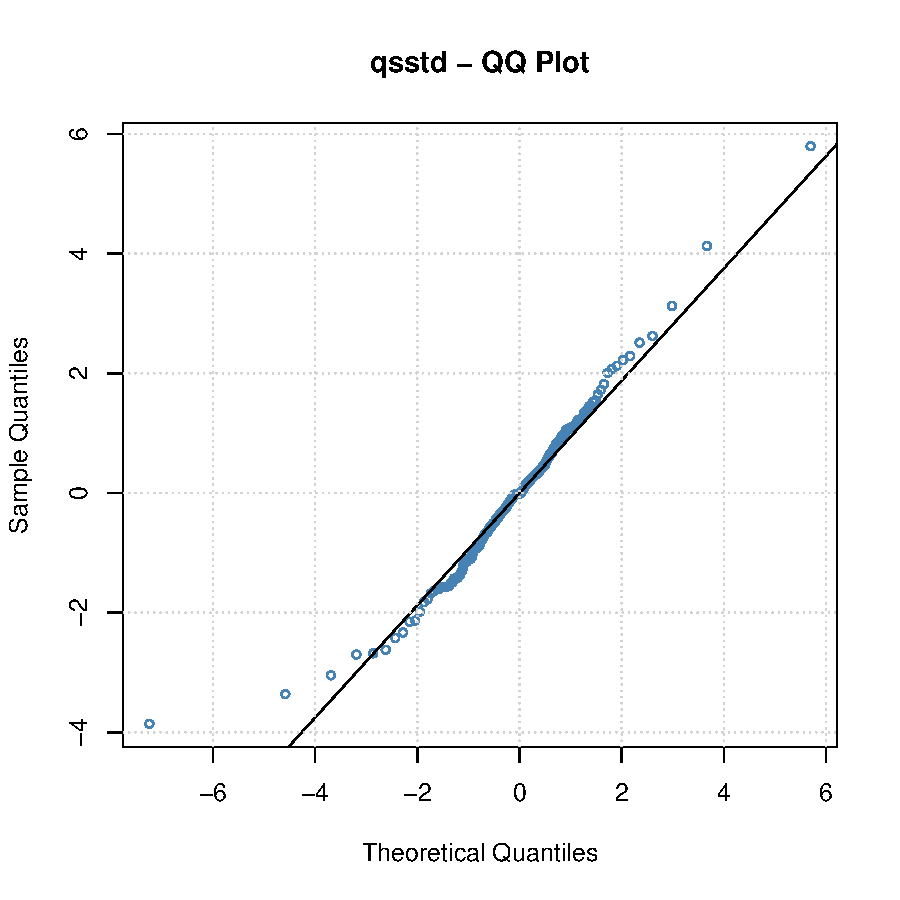
\includegraphics{garch_tests_example-012}

\begin{Schunk}
\begin{Sinput}
R> fit3 <- garchFit(~aparch(1,1), cond.dist = c("sstd"), data = logreturns, trace = FALSE)
R> summary(fit3)
\end{Sinput}
\begin{Soutput}
Title:
 GARCH Modelling 

Call:
 garchFit(formula = ~aparch(1, 1), data = logreturns, cond.dist = c("sstd"), 
    trace = FALSE) 

Mean and Variance Equation:
 data ~ aparch(1, 1)
<environment: 0x55d0fc0789c0>
 [data = logreturns]

Conditional Distribution:
 sstd 

Coefficient(s):
        mu       omega      alpha1      gamma1       beta1       delta  
 0.0041452   0.0327264   0.2478499  -0.0418682   0.8087231   0.3198010  
      skew       shape  
 0.9166215   2.0864552  

Std. Errors:
 based on Hessian 

Error Analysis:
         Estimate  Std. Error  t value Pr(>|t|)    
mu      0.0041452   0.0004216    9.833   <2e-16 ***
omega   0.0327264   0.0181558    1.803   0.0715 .  
alpha1  0.2478499   0.1271906    1.949   0.0513 .  
gamma1 -0.0418682   0.2213966   -0.189   0.8500    
beta1   0.8087231   0.0542195   14.916   <2e-16 ***
delta   0.3198010   0.2885047    1.108   0.2677    
skew    0.9166215   0.0298303   30.728   <2e-16 ***
shape   2.0864552   0.1228352   16.986   <2e-16 ***
---
Signif. codes:  0 ‘***’ 0.001 ‘**’ 0.01 ‘*’ 0.05 ‘.’ 0.1 ‘ ’ 1

Log Likelihood:
 521.1966    normalized:  0.91438 

Description:
 Tue Mar 14 16:08:00 2023 by user: georgi 


Standardised Residuals Tests:
                                Statistic    p-Value  
 Jarque-Bera Test   R    Chi^2  7441750      0        
 Shapiro-Wilk Test  R    W      0.04272342   0        
 Ljung-Box Test     R    Q(10)  1.257269     0.9995135
 Ljung-Box Test     R    Q(15)  1.262074     0.9999987
 Ljung-Box Test     R    Q(20)  1.2943       1        
 Ljung-Box Test     R^2  Q(10)  0.0007368121 1        
 Ljung-Box Test     R^2  Q(15)  0.0007430762 1        
 Ljung-Box Test     R^2  Q(20)  0.0007511647 1        
 LM Arch Test       R    TR^2   6.813758     0.8696717

Information Criterion Statistics:
      AIC       BIC       SIC      HQIC 
-1.800690 -1.739698 -1.801077 -1.776893 
\end{Soutput}
\end{Schunk}

The qq-plots of the standardised results for all models fitted above suggest that the chosen
conditiional distributions are unsatisfactory. Moreover, the fitted standardised-t
distributions have shape parameters (degrees of freedom) slightly over two. Suggesting
extremely heavy tails, maybe even the need for stable distributions.

Note also that in all models above $\alpha_{1} + \beta_{1}$ is greater than one, a possible
violation of any form of stationarity.

Or maybe, it is just that the GARCH models tried here are not able to accomodate varying
behaviour before, during and after the financial crisis.


\end{document}
